\section{Base de datos}
Como ya se ha mencionado anteriormente se ha decidido usar una base
de datos no relacional. A continuación se expondrán las razones
para ello:

\begin{itemize}
    \item Al tratarse de datos no homogéneos en referencia con los
    ejercicios, pues estos pueden tener o no varios pasos, pueden
    tener o no material visual en forma de imágenes o vídeos. Esto
    ocurre debido a que no están digitalizados de forma alguna a día
    de hoy y el propio cliente no sabe como lo hará.
    \item Siguiendo con el punto anterior los propios usuarios
    no son consistentes. Existen dos tipos de usuarios y cada
    uno de ellos tiene relaciones distintas
    con los ejercicios y con los propios usuarios, es por ello que
    las bases de datos no relacionales (NoSQL) presentan una mejora
    respecto de las relacionales.
    \item Otro punto a tener en cuenta ha sido el tener que trabajar
    con eventos de tiempo, dejar marcas temporales en el instante en
    el que se ha completado un ejercicio. Esto se soluciona de forma
    más fácil con este tipo de base de datos.
    \item Por otro lado esta aplicación no presenta complejidad en
    peticiones a la base de datos en un primer momento, esta se
    enfoca más en peticiones de "grandes" cantidades de datos la
    mayor parte del tiempo, esto hace que no se pueda aprovechar la
    potencia de las peticiones SQL \cite{sql}.
    \item Una de las funcionalidades que se pedía implementar en el
    proyecto es un sistema de mensajería interna (chat) por el que
    poder comunicarse doctores con pacientes y viceversa, esta
    funcionalidad es más sencilla solventarla en bases de datos no
    relacionales.
\end{itemize}

\medskip
Por estas razones se ha decidido usar un sistema de base de datos
no relacional como es el que nos provee \textit{firebase}. Además
para el registro de usuarios se ha usado el módulo de autenticación
del que dispone esta misma plataforma, el cual permite el registro
de usuarios por múltiples vías si así lo quisiéramos, guardan de
forma segura las contraseñas e incorpora un sistema de verificación
de correo en el momento del registro. Es por ello que se ha tenido
que crear un objeto en la base de datos, a parte del existente,
para incluir datos personales que usando este módulo no nos permitían
guardar. Para ello se ha creado un grupo llamado \textit{users} donde
crear objetos de nombre, el identificador único, generados en el
momento del registro de cada usuario y dentro de este el resto de
datos que nos han sido necesarios.

\medskip
\begin{figure}
    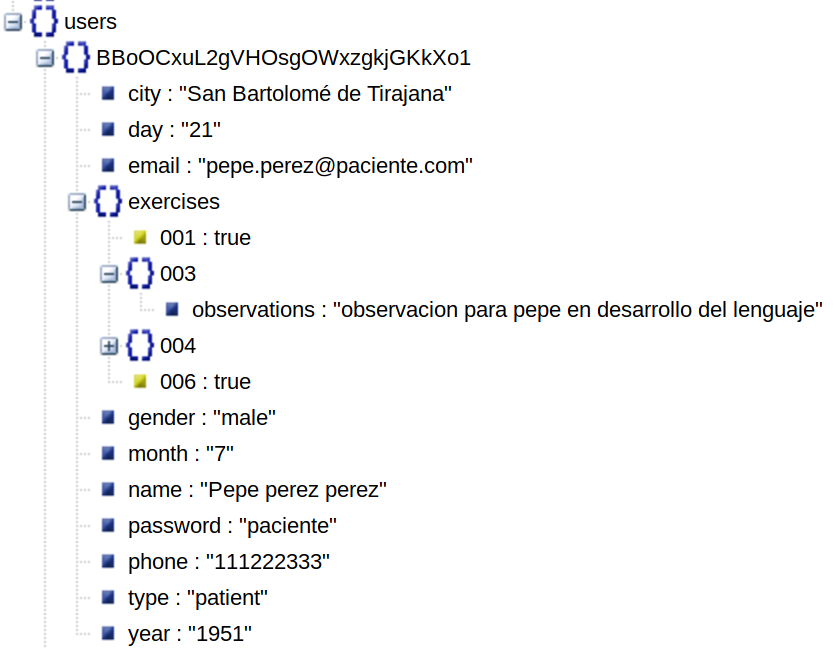
\includegraphics[width=\linewidth]{./images/database/users-patient-with-observations-database.png}
    \caption{Estructura en la base de datos del objeto: usuarios (con observaciones en los ejercicios)}
    \label{usuario-con-observaciones}
\end{figure}

Como se puede ver en la \textbf{figura \ref{usuario-con-observaciones}},
los usuarios comparten parámetros comunes de los cuales solamente los que
se explicarán a continuación pueden generar duda de su utilidad o uso que se
le ha podido dar. Es el caso de \textit{city}, hace referencia a la ciudad de
nacimiento del usuario y por otro lado el trío \textit{day-month-year} los
cuales forman la fecha de nacimiento del usuario en cuestión.
En este caso el usuario tiene asignados cuatro ejercicios dentro del objeto
\textit{exercise} a los cuales se les "referencia" guardando su ID y en caso
de que este tenga observaciones con este paciente, se le añade un parámetro
interno \textit{observations}.


\medskip
\begin{figure}
    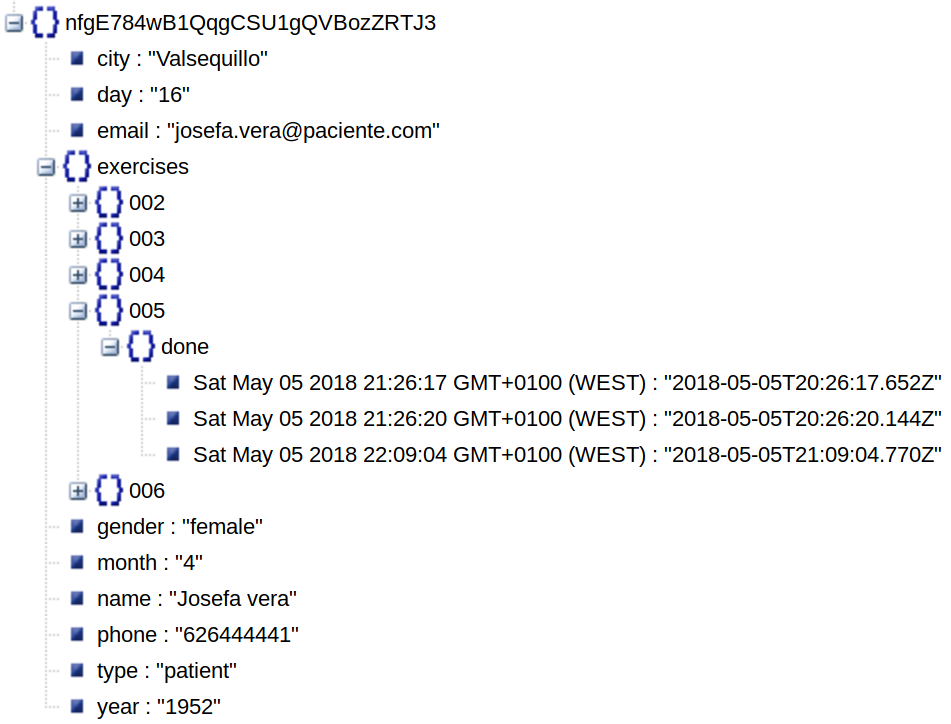
\includegraphics[width=\linewidth]{./images/database/users-patient-with-exercises-done-database.png}
    \caption{Estructura en la base de datos del objeto: usuarios (con ejercicios completados)}
    \label{usuario-con-ejercicios}
\end{figure}

En esta \textbf{figura \ref{usuario-con-ejercicios}} queda reflejado como
se guardan las veces que se marca un ejercicio como hecho, guardando como clave
del parámetro un objeto de tipo fecha y como valor el mismo pero en ristra de
caracteres.

\medskip
\begin{figure}
    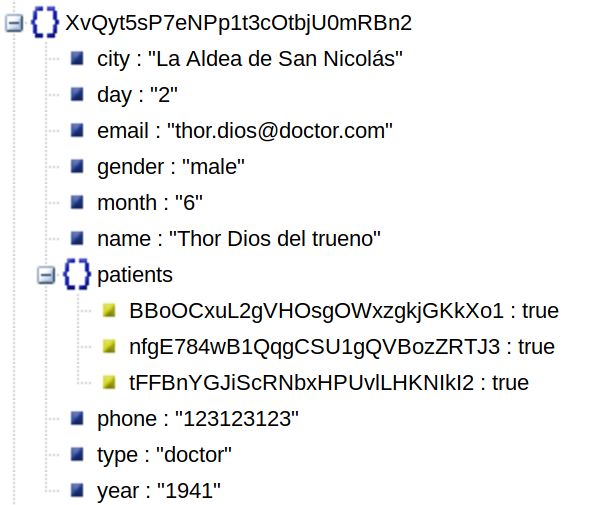
\includegraphics[width=\linewidth]{./images/database/users-doctor-database.png}
    \caption{Estructura en la base de datos del objeto: usuarios (doctor)}
    \label{usuario-doctor}
\end{figure}

En caso de ser un usuario de tipo doctor este tendrá un objeto en el que
guarda los identificadores de sus pacientes asignados, como se puede ver
en la \textbf{figura \ref{usuario-doctor}}.

\medskip
\begin{figure}
    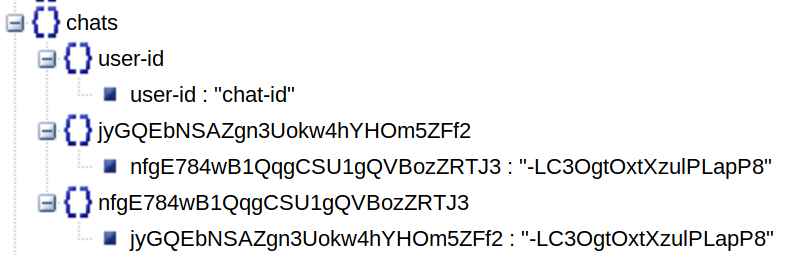
\includegraphics[width=\linewidth]{./images/database/chats-database.png}
    \caption{Estructura en la base de datos del objeto: chats}
    \label{chat}
\end{figure}

Para no hacer grandes cantidades de peticiones sin necesidad
se ha creado un objeto \textit{chats}, el cual se puede ver en la
\textbf{figura \ref{chat}}. Para explicar mejor como están estructurados
estos datos se pondrá un ejemplo. Si un usuario \textbf{A} tiene un chat
iniciado con un usuario \textbf{B} en la base de datos en la parte de chat
aparecerá la siguiente información:

\smallskip
\textit{chats/ ID-usuario-A/ [ID-usuario-B: ID-chat]}

\smallskip
\textit{chats/ ID-usuario-B/ [ID-usuario-A: ID-chat]}

\smallskip
En caso de que un tercer usuario \textbf{C} inicie un chat con \textbf{A}
aparecerá una nueva entrada y quedará de la siguiente forma la base de datos:

\smallskip
\textit{chats/ ID-usuario-A/ [ID-usuario-B: ID-chat], [ID-usuario-C: ID-chat]}

\smallskip
\textit{chats/ID-usuario-B/[ID-usuario-A: ID-chat]}

\smallskip
\textit{chats/ID-usuario-C/[ID-usuario-A: ID-chat]}

\smallskip
Como se ha dicho esto se ha realizado de esta forma para ahorrar
tener que traer todos los
mensajes del chat en caso de que un usuario solo quiera visualizar con
que personas tiene un chat abierto, de esta forma solo hará una petición
al objeto con su identificador y este le devolverá los ID de los usuarios
con los que mantiene la conversación y el ID del chat en cuestión si quiere
obtener los mensajes.

\medskip
\begin{figure}
    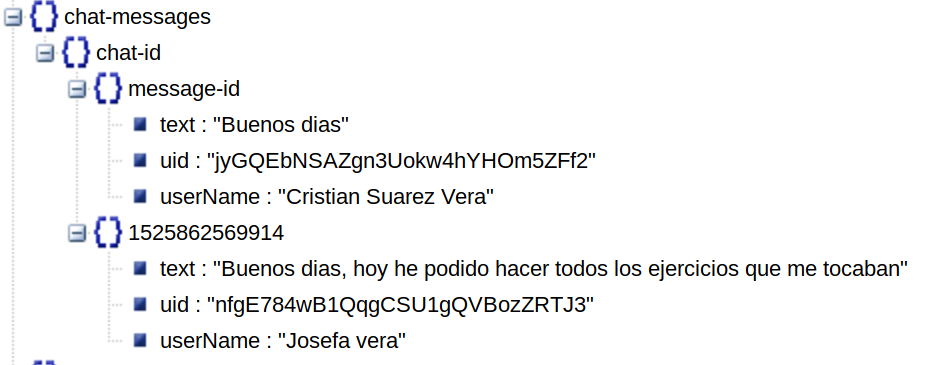
\includegraphics[width=\linewidth]{./images/database/chat-messages-database.png}
    \caption{Estructura en la base de datos del objeto: mensajes del chat}
    \label{mensajes-del-chat}
\end{figure}

A raíz de la implementación anterior se ha tenido que crear el objeto
que muestra la \textbf{figura \ref{mensajes-del-chat}}, este tiene como
objetivo almacenar todos los mensajes de los chats entre los distintos
usuarios. Cada chat tiene su identificador único con el que se crea el
objeto y dentro de este un identificador de mensaje el cual internamente
tiene el mensaje que ha sido enviado, el identificador del usuario que
ha enviado el mensaje y el nombre completo del usuario que ha enviado
el mensaje. Este último parámetro puede parecer redundante pero nos
ahorra posteriormente, a la hora de mostrar los mensajes, tener que hacer
una petición al servidor para obtener este dato.

\medskip
\begin{figure}
    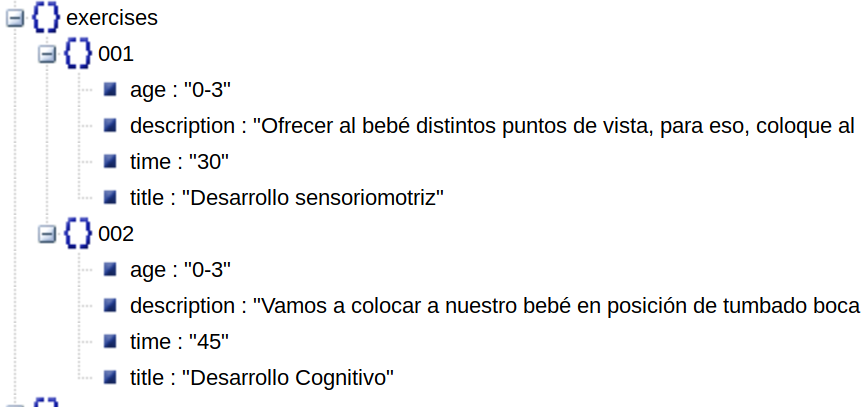
\includegraphics[width=\linewidth]{./images/database/exercises-database.png}
    \caption{Estructura en la base de datos del objeto: ejercicios}
    \label{ejercicios}
\end{figure}

Por último en la \textbf{figura \ref{ejercicios}} se ve
como se ha creado el objeto para los ejercicios. En él se almacena la información
referente a cada ejercicio como puede ser la edad recomendada del ejercicio,
la descripción del mismo, el tiempo medio que se tarda en realizarlo y el
título que este tiene. Además todo ello está bajo un objeto que tiene como
nombre un identificador único para el ejercicio.

% Diseño arquitectonico el que viene con ionic por defecto, mirar cual es